\section{Evaluation}
We evaluate the following sequential selection baselines:
\begin{itemize}\addtolength{\itemsep}{-.35\baselineskip}
\item \textbf{Static, greedy}: corresponds to best performance of a policy that does not observe feature values and selects actions greedily ($\gamma=0$).
\item \textbf{Static, non-myopic}: policy that does not observe feature values but uses the MDP machinery with $\gamma=1$ to consider future action rewards.
\item \textbf{Dynamic, greedy}: policy that observed feature values, but selects actions greedily.
% \item \todo{
% \textbf{Active Classification} \parencite{Gao-NIPS-2011}:
% Feature selection is done by greedy selection based on expected information gain divided by cost (so reward is information gain, $\gamma=0$).
% The feature responses are modeled as a mixture of multivariate Gaussians (one mixture element per class label), and inference is instance-specific, akin to locally weighted regression.
% Feature combination is done by the same model: the posteriors are used as the final answers.
% }
% \item
% \todo{\textbf{MD-DAG} \parencite{Benbouzid-ICML-2012}
% Feature selection is done by an MDP policy with three actions: Skip, Evaluate, Quit over a pre-determined sequence of weak learners (unspecified exactly how the sequence is arranged, except ``by quality'').
% }
\end{itemize}
Our method is the \textbf{Dynamic, non-myopic} policy: observed feature values, and full lookahead.

% In addition to the settings above, we evaluate three additional baselines that do not do any selection at all: (a) \textbf{all} features computed; (b) only the \textbf{best} feature (in terms of $\mathcal{G}$) computed; (c) only the \textbf{least costly} feature computed.

In preliminary experiments, Logistic Regression always performed better than the Gaussian Naive Bayes classifier, and so only the former is used in the experiments below.
As described above, we evaluated classification with \textbf{Gaussian} vs. \textbf{Mean} imputation, and with different number of classifiers (1, 3, and 6) clustered by feature subsets.
We found that mean imputation performed better than Gaussian imputation, and although increased number of classifiers sometimes increased performance, it also made our method more prone to overfitting; $K=1$ classifiers worked best on all tasks.
%For reason of space, we report only the best achieved performance in the following evaluation results.

We evaluate two forms of test-time efficient performance measure: the area under the curve and the performance at max budget, although note that all methods are trained only for the former measure.

While the individual implementation details have been largely provided in the preceding text, here we additionally note that some of our policy and classifier implementations use the scikit-learn package \parencite{Pedregosa2011}.

% \subsection{Baselines}
% \paragraph{Active Classification \parencite{Gao-NIPS-2011}}
% Feature selection is done by greedy selection based on expected information gain divided by cost (so reward is information gain, $\gamma=0$).
% The feature responses are modeled as a mixture of multivariate Gaussians (one mixture element per class label), and inference is instance-specific, akin to locally weighted regression.
% Feature combination is done by the same model: the posteriors are used as the final answers.

% \paragraph{Greedy Miser \parencite{Xu-ICML-2012}}
% Feature selection is done by the CART algorithm \parencite{Breiman-1984} with an impurity function that considers feature cost.
% Feature combination is an ensemble of trees.

% \paragraph{MD-DAG \parencite{Benbouzid-2012-ICML}}
% Feature selection is done by an MDP policy with three actions: Skip, Evaluate, Quit over a pre-determined sequence of weak learners (unspecified exactly how the sequence is arranged, except ``by quality'').
% Feature combination is an unweighted sum.

% \paragraph{Timely \parencite{Karayev-NIPS-2012}}
% Feature selection is done by MDP trained using a state feature vector that has the inference output of an MRF combining feature values.
% Feature combination is done by the same MRF.

\begin{figure*}[ht]
\centering
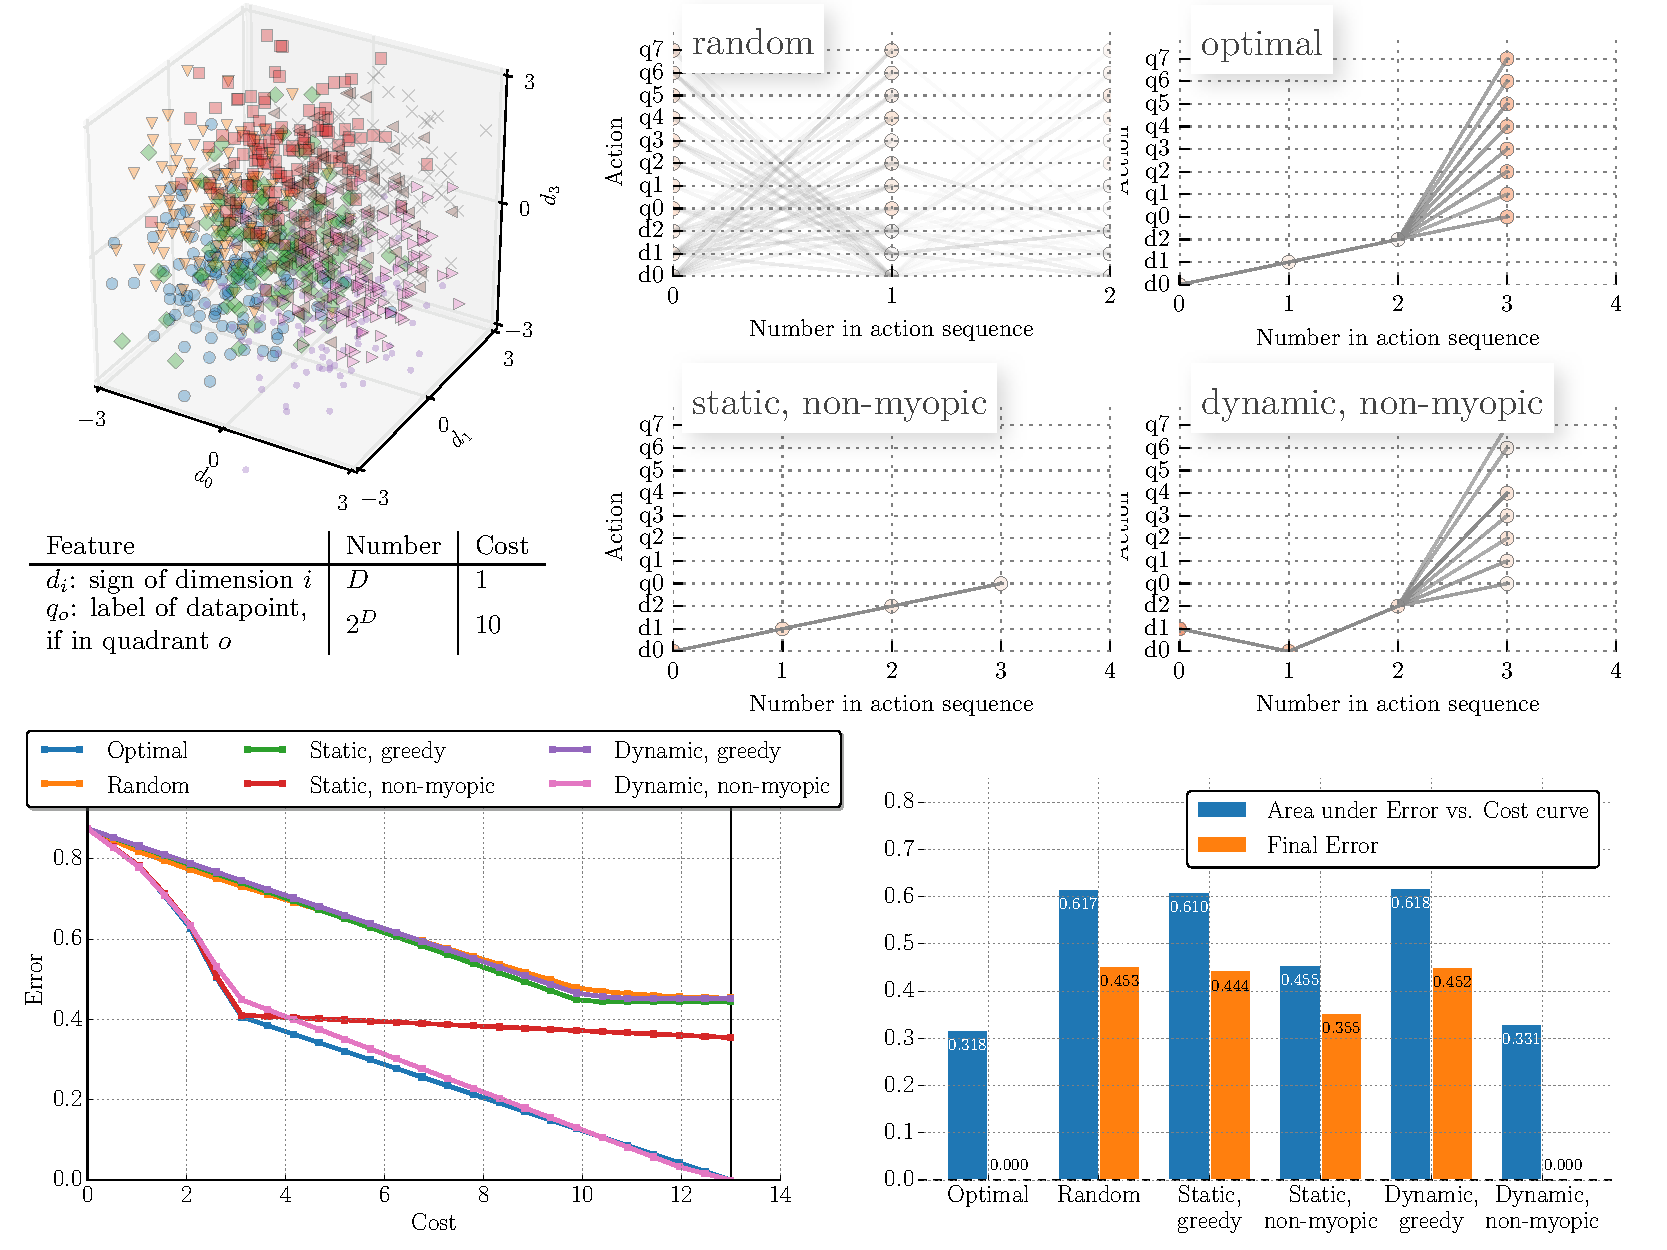
\includegraphics[width=.9\textwidth]{../../figures/synthetic.pdf}
\caption{
Evaluation on the synthetic example (best viewed in color).
The data and the feature costs are shown at top left; the sample feature trajectories of different policies at top right.
(The opacity of the edges corresponds to their prevalence during policy execution; the opacity of the nodes corresponds to the amount of reward obtained in that state.)
Note that the \emph{static, non-myopic} policy correctly learns to select the cheap features first, but is not able to correctly branch, while our \emph{dynamic, non-myopic} approach finds the optimal strategy.
The plots in the bottom half give the error vs. cost numbers.
}

\label{fig:synthetic}
\end{figure*}

\subsection{Synthetic Experiment.}
Following \parencite{Xu-ICML-2013}, we first show that the policy works as advertised in a challenging synthetic example.
In $D$-dimensional space, the data has a label for each of the $2^D$ orthants, and is generated by a unit-variance Gaussian in that orthant (See top left of \autoref{fig:synthetic} for the 3D case).
There are $D$ cheap features that simply return the sign of the data point's coordinate for the corresponding dimension.
For each orthant, there is also an expensive feature that returns the data point's label if the point is located in the corresponding orthant, and random noise otherwise.

The optimal policy on a new data point is to determine its orthant with cheap features, and then take the corresponding expensive action.
Note that both dynamic features and non-myopic learning are crucial to the optimal policy, which is successfully found by our approach.
\autoref{fig:synthetic} shows the results of this optimal policy, a random policy, and of different baselines and our method, trained given the correct minimal budget.

\subsection{Scene recognition.}
The Scene-15 dataset \parencite{Lazebnik-CVPR-2006} contains 4485 images from 15 visual scene classes.
The task is to classify images according to scene.
Following \parencite{Xiao-CVPR-2010}, we extracted 14 different visual features (GIST, HOG, TinyImages, LBP, SIFT, Line Histograms, Self-Similarity, Textons, Color Histograms, and variations).
The features vary in cost from 0.3 seconds to 8 seconds, and in single-feature accuracy from 0.32 (TinyImages) to .82 (HOG).
Separate multi-class linear SVMs were trained on each feature channel, using a random 100 positive example images per class for training.
We used the \texttt{liblinear} implementation, and K-fold cross-validated the penalty parameter $C$.
The trained SVMs were evaluated on the images not used for training, resulting in a dataset of 2238 vectors of 210 confidence values: 15 classes for each of the 14 feature channels.
This dataset was split 60-40 into training and test sets for our experiments.

\hyperref[fig:scenes]{Figure~\ref*{fig:scenes}} shows the results, including learned policy trajectories.
For all evaluated budgets, our \emph{dynamic, non-myopic} method outperforms all others on the area under the error vs. cost curve metric.
Our results on this dataset match the reported results of Active Classification \parencite{Gao-NIPS-2011} (Figure 2) and Greedy Miser \parencite{Xu-ICML-2012} (Figure 3), although both methods use an additional powerful feature channel (ObjectBank)\footnote{Detailed results for this and other experiments are on the project page (see front page for the \href{http://sergeykarayev.com/recognition-on-a-budget/}{link}).}.


\subsection{ImageNet and maximizing specificity.}
The full ImageNet dataset has over 10K categories and over a million images \parencite{Deng-ECCV-2010}.
The classes are organized in a hierarchical structure, which can be exploited for novel recognition tasks.
We evaluate on a 65-class subset introduced in ``Hedging Your Bets'' \parencite{Deng-CVPR-2012}.
In this evaluation, we consider the situation where the initial feature computation has already happened, and the task is to find a path through existing one-vs-all classifiers: features correspond to Platt-scaled SVM confidences of leaf-node classifiers (trained on SIFT-LLC features), and each has cost 1 \parencite{Deng-ECCV-2010}.
Following \parencite{Deng-CVPR-2012}, accuracy is defined on all nodes, and inner node confidences are obtained by summing the probabilities of the descendant nodes.

We combine our sequential feature selection with the ``Hedging Your Bets'' method for backing off prediction nodes using the ImageNet hierarchy to maintain guaranteed accuracy while giving maximally specific answers, given a cost budget.
The results are given in \hyperref[fig:imagenet]{Figure~\ref*{fig:imagenet}}.
As the available budget increases, the \emph{specificity} (defined by normalized information gain in the hierarchy) of our predictions also increases, while accuracy remains constant.
Visualizing this on the ILSVRC-65 hierarchy, we see that the fraction of predictions at the leaf nodes grows with available computation time.
This formulation presents a novel angle on modeling the time course of human visual perception.

\begin{figure*}[ht]
\centering
    \centering
    \begin{subfigure}[b]{0.39\textwidth}
            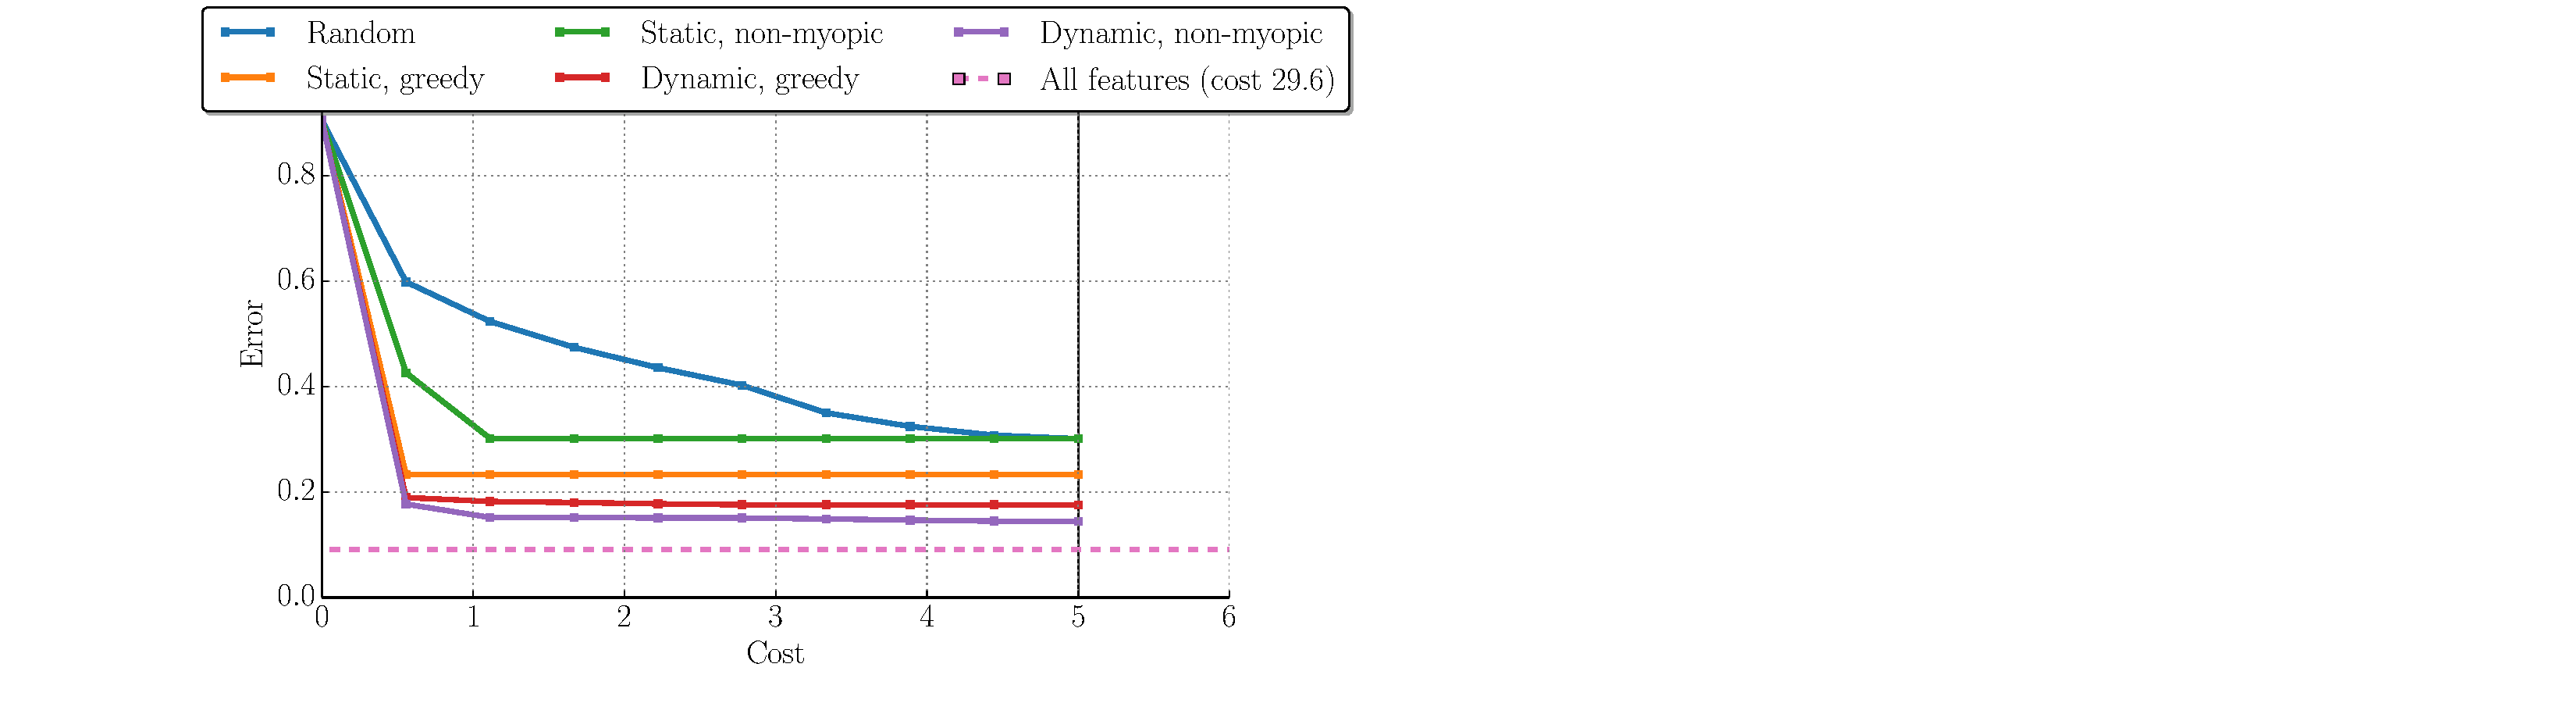
\includegraphics[width=\textwidth]{../../figures/apr11_assembly/scene_15_5_crop.pdf}
            \caption{Error given by policies learned for a budget = 5.}
    \end{subfigure}%
    \begin{subfigure}[b]{0.36\textwidth}
            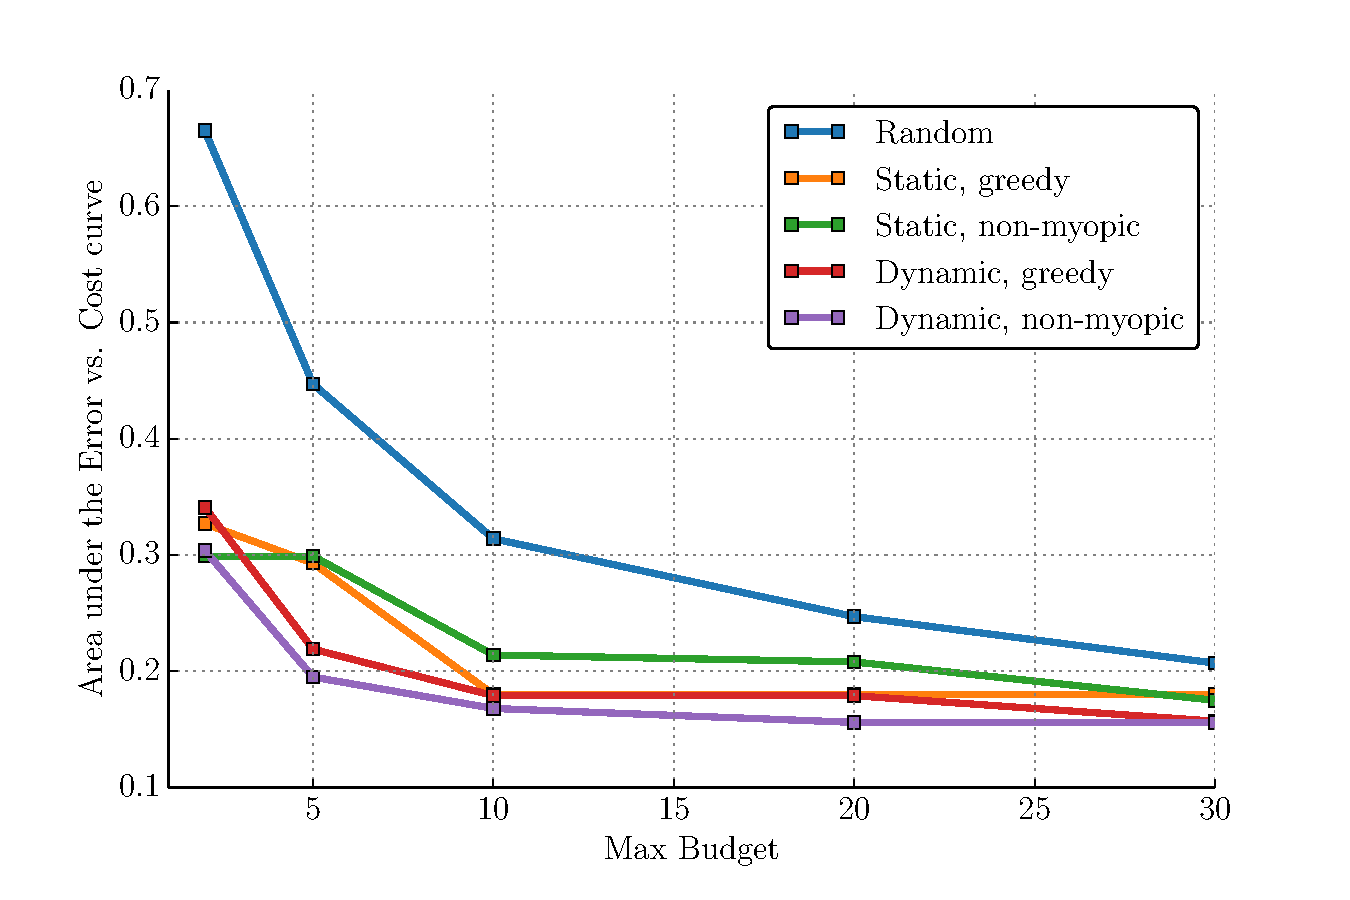
\includegraphics[width=\textwidth]{../../figures/apr11_assembly/_scenes15_auc.pdf}
            \caption{Areas under error vs. cost curves of policies learned at different budgets.}
    \end{subfigure}%
    \begin{subfigure}[b]{0.25\textwidth}
            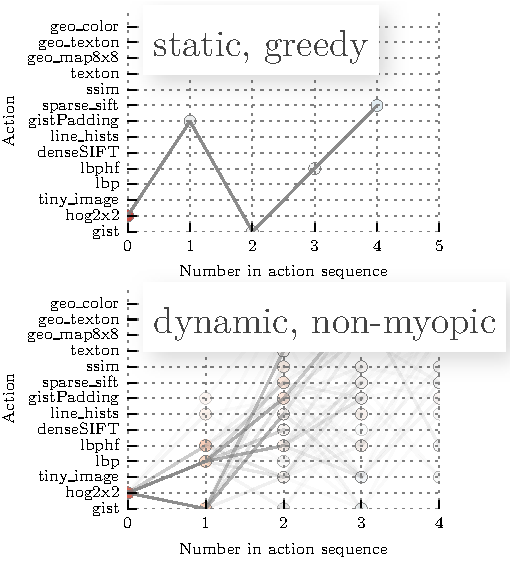
\includegraphics[width=\textwidth]{../../figures/apr11_assembly/scenes_result.pdf}
            \caption{Policy trajectories.}
    \end{subfigure}

    \caption{
Results on Scenes-15 dataset (best viewed in color).
Figure (a) shows the error vs. cost plot for policies learned given a budget of 5 seconds.
Figure (b) aggregates the area under the error vs. cost plot metrics for different policies and budgets, showeing that our approach outperforms baselines no matter what budget it's trained for.
Figure (c) shows the branching behavior of our dynamic policy.
\label{fig:scenes}
    }
\end{figure*}
\begin{figure*}[ht]
\centering
    \begin{subfigure}[b]{0.52\textwidth}
            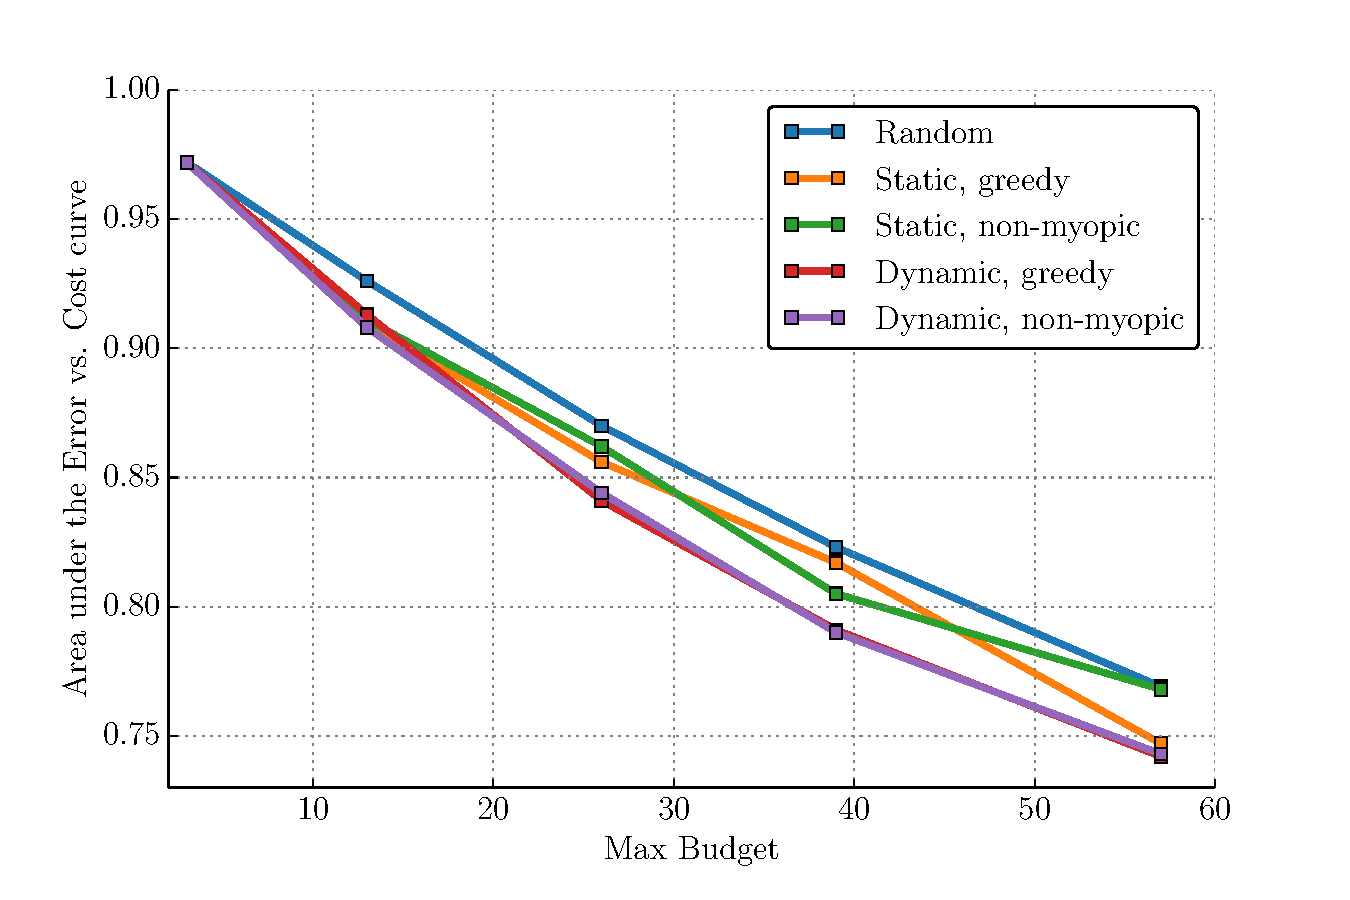
\includegraphics[width=\textwidth]{../../figures/apr11_assembly/_ilsvrc65_auc.pdf}
            \caption{
            Areas under error vs. cost curves for policies learned at different budgets.
            (No specificity back-off is performed here).
            \label{fig:imagenet-a}
            }
    \end{subfigure}\hfill%
    \begin{subfigure}[b]{0.43\textwidth}
            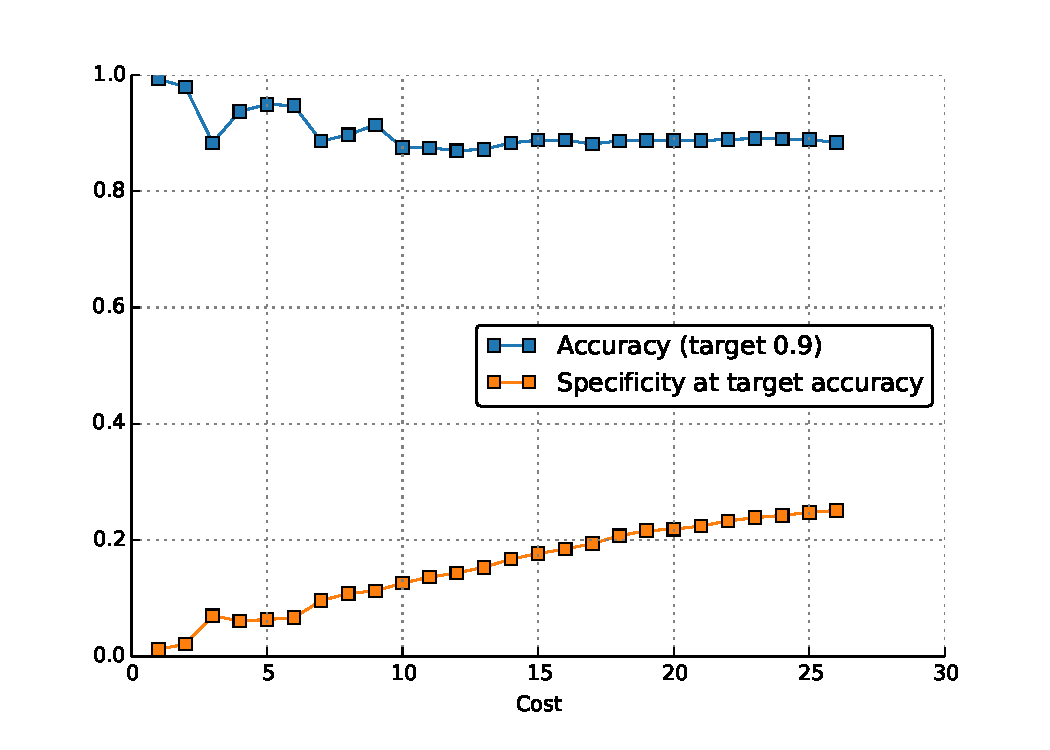
\includegraphics[width=\textwidth]{../../figures/apr11_assembly/ilsvrc65_acc.pdf}
            \caption{
            Holding prediction accuracy constant, we achieve increased specificity with increased cost (on \emph{Dynamic, non-myopic} policy, budget = 36).
            \label{fig:imagenet-b}
            }
    \end{subfigure}\\\vspace{1em}
    \begin{subfigure}[b]{.97\textwidth}
            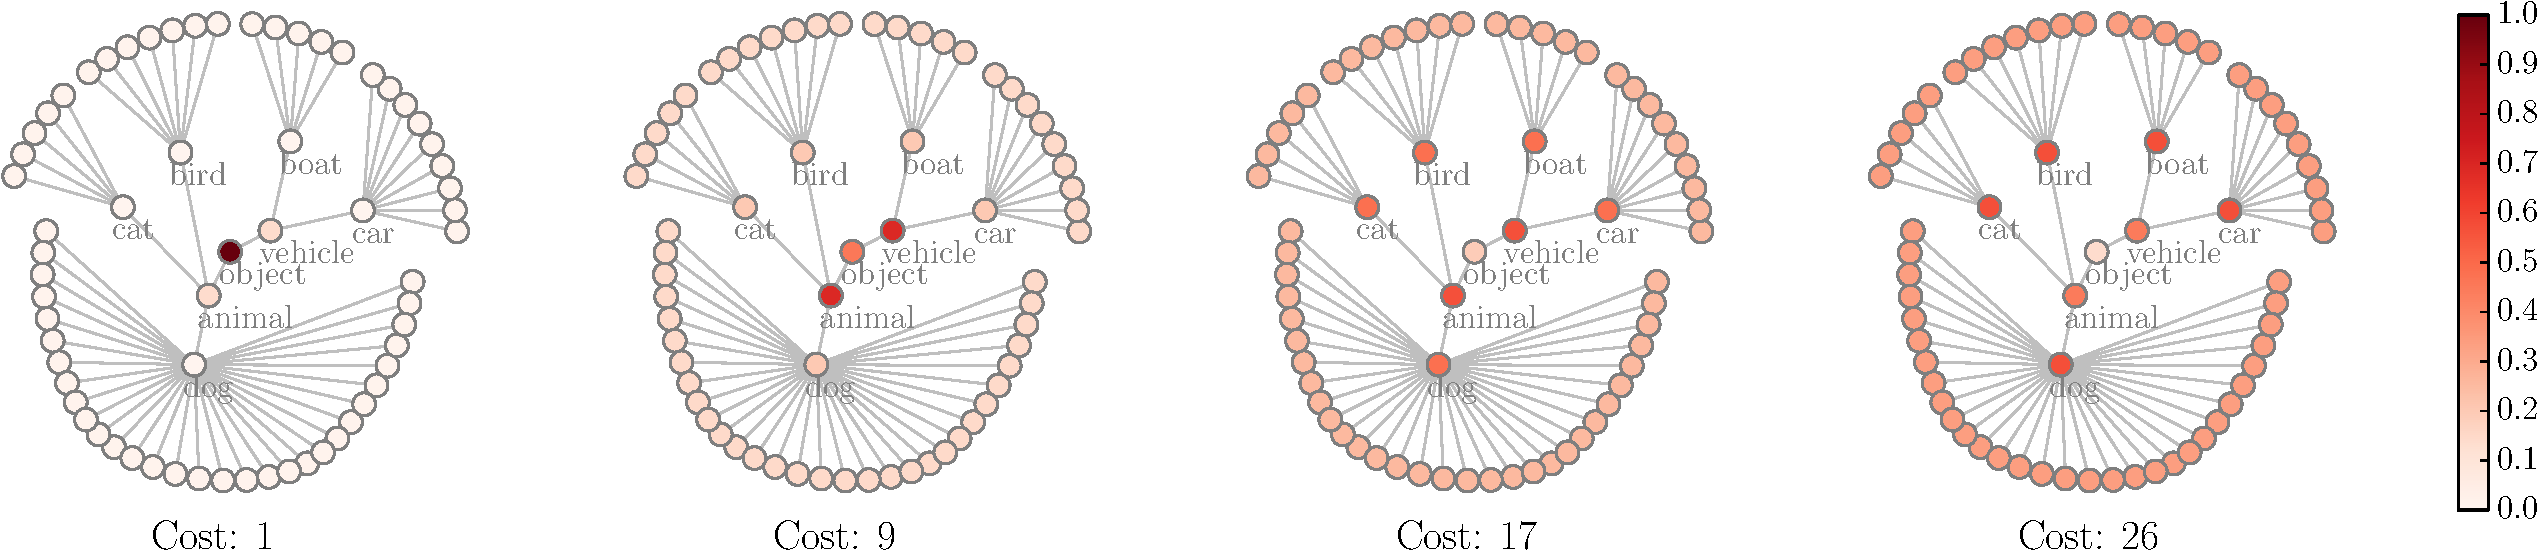
\includegraphics[width=\textwidth]{../../figures/apr11_assembly/ilsvrc65_network-crop.pdf}
            \caption{
            We visualize the fraction of predictions made at inner vs. leaf nodes of ILSVRC-65 at different cost points of an Anytime policy: with more computation, accurate predictions are increasingly made at the leaf nodes.
            \label{fig:imagenet-c}
            }
    \end{subfigure}

\caption{
Results on the ILSVRC-65 dataset (best viewed in color).
Figure (a) shows our dynamic approaches outperforming static baselines for all practical cost budgets.
When our method is combined with Hedging Your Bets \parencite{Deng-CVPR-2012}, a constant prediction accuracy can be achieved at all points in the Anytime policy, with \emph{specificity} of predictions increasing with the cost of predictions.
Figures (b) and (c) show this for the \emph{dynamic, non-myopic} policy learned for budget = 26.
This is analogous to human visual performance, which shows increased specificity at longer stimulus times.
\label{fig:imagenet}}
\end{figure*}
